\chapter{Results} \label{chap:results}

This chapter contains waveforms and plots referent to the tests realized to determine the driving ability of the \ac{WMU} and their explanations. The tests were realized on the in-wheel motor by applying two types of driving methods: trapezoidal and sinusoidal, both at open loop and closed loop. These driving methods were tested under two conditions: loaded and unloaded. 

The power was supplied by an Elind KL Series power supply with a current limit of 15 A. The analog signals were obtained by a Rigol oscilloscope, model $DS1054$. The speed readings were obtained through the implemented LabView \ac{UI}. All the plots and waveforms were processed in Matlab for their analysis.

\section{Trapezoidal Drive -- Open Loop}

The trapezoidal open loop driving was executed by setting a duty cycle directly into the six-step sequence \ac{PWM}. The algorithm was executed at $50kHz$ and the \ac{PWM} signal has a frequency of $15kHz$.

Figure \ref{fig:plot1} shows the different speeds achievable by applying different duty cycles with different torque loads. The curves on the plot start on different duty cycles since the torque load couldn’t reach a steady value until a certain speed was stablished. For example, for the measurement with a load equal to $3 Nm$, the curve starts at a duty cycle equal to $30\%$, since at a duty cycle lower than this or a speed lower than $10 rad/s$, the load can’t be generated by the test bench, which would apply around $2 Nm$, therefore those measurements were not considered for the plot. On the other hand, the curves that don’t show large duty cycle values ($5$ and $6 Nm$), is because the power supply couldn’t feed enough current to the driver to reach such torque.

Figures \ref{fig:trap_v1}, \ref{fig:trap_v2}, \ref{fig:trap_v3} and \ref{fig:trap_v4} show the voltage waveforms measured on the terminals of the motor. The trapezoidal \ac{BEMF} generated on its coils due to the six-step sequence algorithm can be identified as the ramp-up and ramp-down signals between rectangular drives, mainly when the duty cycle is 100\%. From these figures we can also identify that when the load increases, the speed of the motor decreases since there is no speed control loop.

Figures \ref{fig:trap_c1}, \ref{fig:trap_c2}, \ref{fig:trap_c3} and \ref{fig:trap_c4} show the current waveforms. We can see from its shape, mainly when the duty cycle is 100\%, that the \ac{BEMF} of the motor is sinusoidal, even if the trapezoidal drive is applied. As the load increases, along with the reduction of the speed, the current consumption increases. It can also be appreciated that the current waveforms present a larger ripple as the duty cycle and the load increase, which represents a torque ripple that reduces the performance of the motor.

\vfill
\begin{figure}[htbp]
\centering
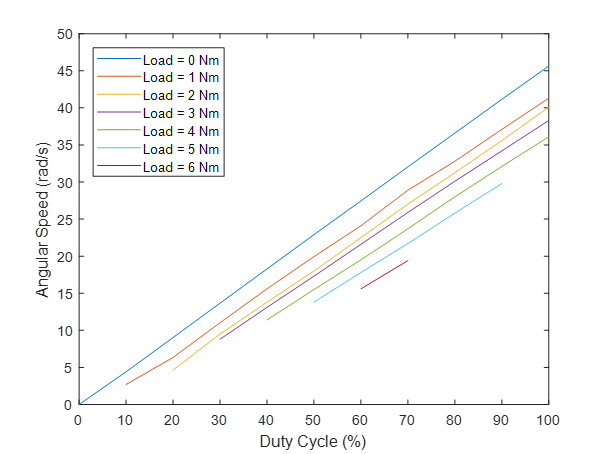
\includegraphics[width=\textwidth]{Images/plots/plot_1.png} 
\caption[Angular Speed vs Duty Cycle at Different Loads]{Plot of the different speeds achieved applying a known duty cycle using an open loop trapezoidal drive with different loads}
\label{fig:plot1}
\end{figure}
\vfill

\begin{figure}[h!p]
\centering
	\subfloat[Duty Cycle = 10\%\label{subfig-1:trap1v}]{%
  		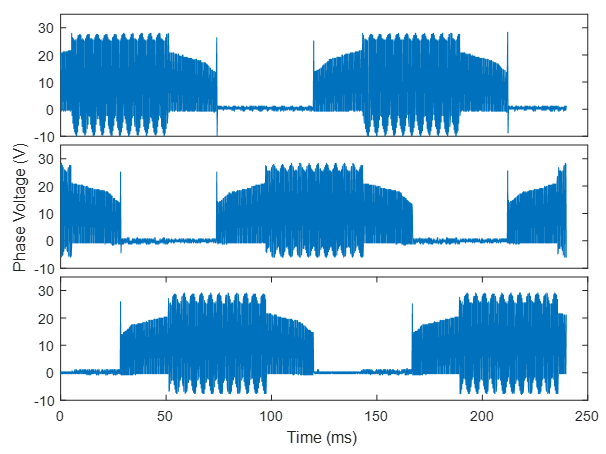
\includegraphics[clip,width=8cm]{Images/waveforms/trap_1.png}%
	}

	\subfloat[Duty Cycle = 50\%\label{subfig-2:trap2v}]{%
  		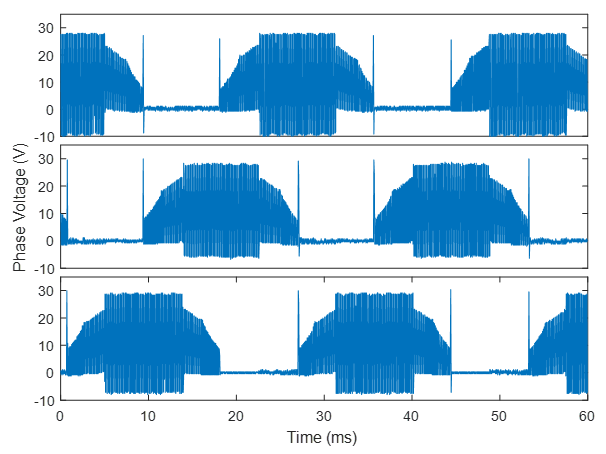
\includegraphics[clip,width=8cm]{Images/waveforms/trap_2.png}%
	}

	\subfloat[Duty Cycle = 100\%\label{subfig-3:trap3v}]{%
  		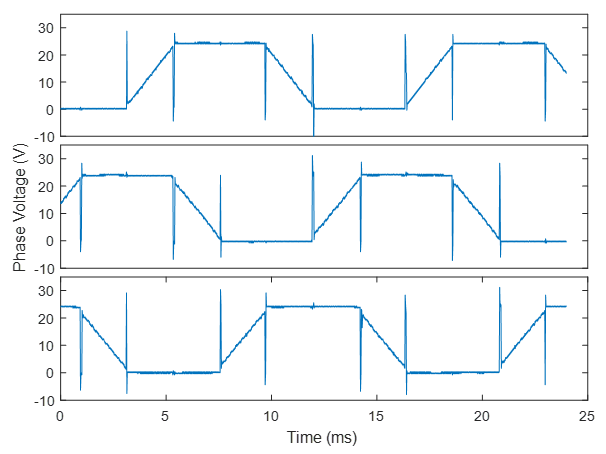
\includegraphics[clip,width=8cm]{Images/waveforms/trap_3.png}%
	}
\caption{Trapezoidal drive voltage waveforms without load applied}
\label{fig:trap_v1}
\end{figure}

\begin{figure}[h!p]
\centering
	\subfloat[Duty Cycle = 10\%\label{subfig-1:trap4v}]{%
  		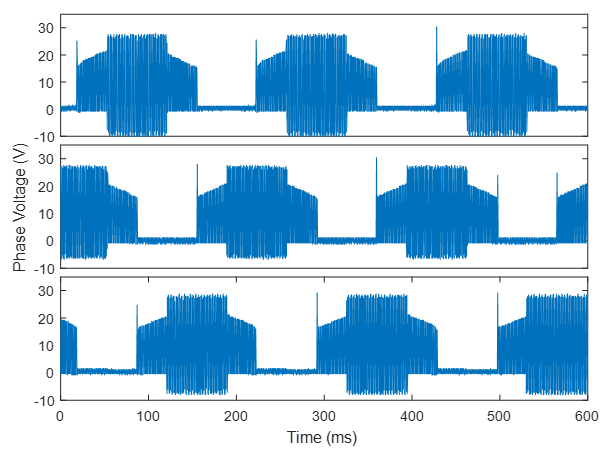
\includegraphics[clip,width=8cm]{Images/waveforms/trap_4.png}%
	}

	\subfloat[Duty Cycle = 50\%\label{subfig-2:trap5v}]{%
  		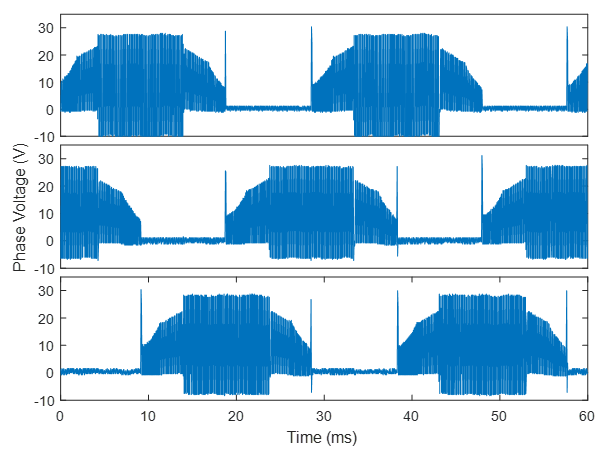
\includegraphics[clip,width=8cm]{Images/waveforms/trap_5.png}%
	}

	\subfloat[Duty Cycle = 100\%\label{subfig-3:trap6v}]{%
  		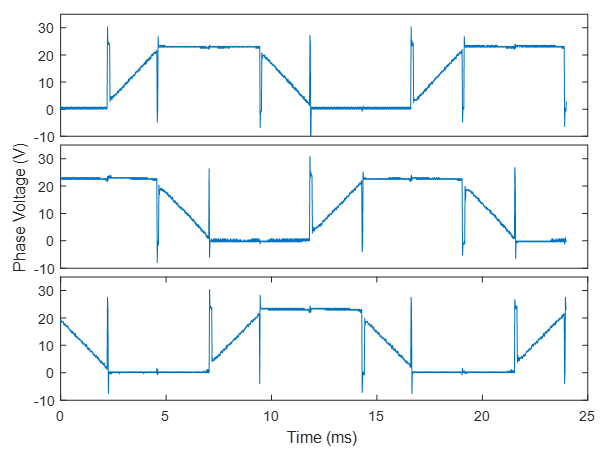
\includegraphics[clip,width=8cm]{Images/waveforms/trap_6.png}%
	}
\caption{Trapezoidal drive voltage waveforms with load = 1 Nm}
\label{fig:trap_v2}
\end{figure}

\begin{figure}[h!p]
\centering
	\subfloat[Duty Cycle = 50\%\label{subfig-1:trap7v}]{%
  		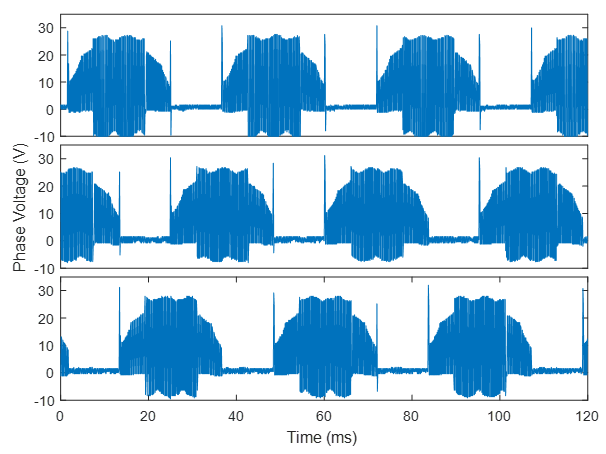
\includegraphics[clip,width=8cm]{Images/waveforms/trap_7.png}%
	}

	\subfloat[Duty Cycle = 100\%\label{subfig-2:trap8v}]{%
  		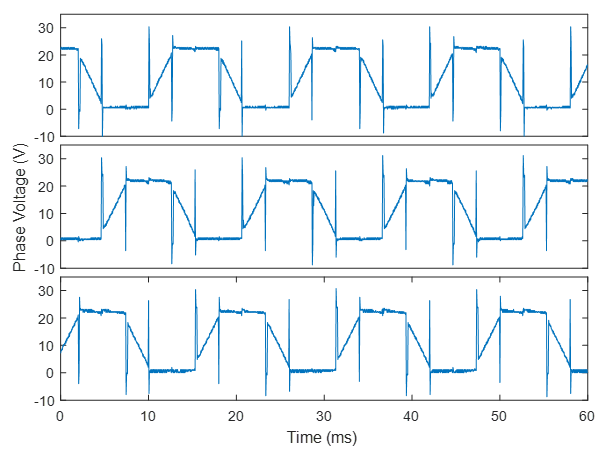
\includegraphics[clip,width=8cm]{Images/waveforms/trap_8.png}%
	}
\caption{Trapezoidal drive voltage waveforms with load = 3 Nm}
\label{fig:trap_v3}
\end{figure}

\begin{figure}[h!p]
\centering
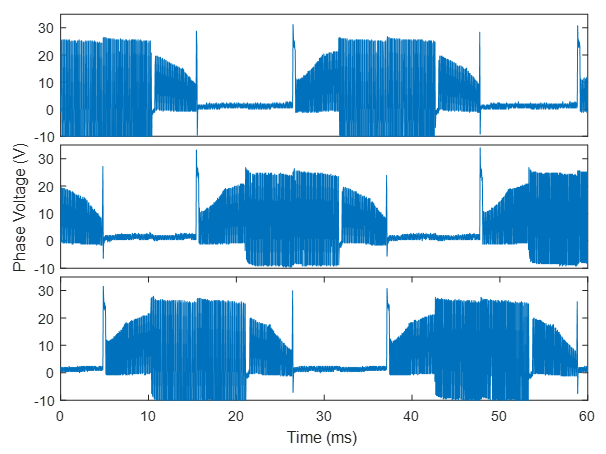
\includegraphics[width=8cm]{Images/waveforms/trap_9.png} 
\caption{Trapezoidal voltage waveforms drive Duty Cycle = 70\% and load = 6 Nm}
\label{fig:trap_v4}
\end{figure}

\begin{figure}[h!p]
\centering
	\subfloat[Duty Cycle = 10\%\label{subfig-1:trap1c}]{%
  		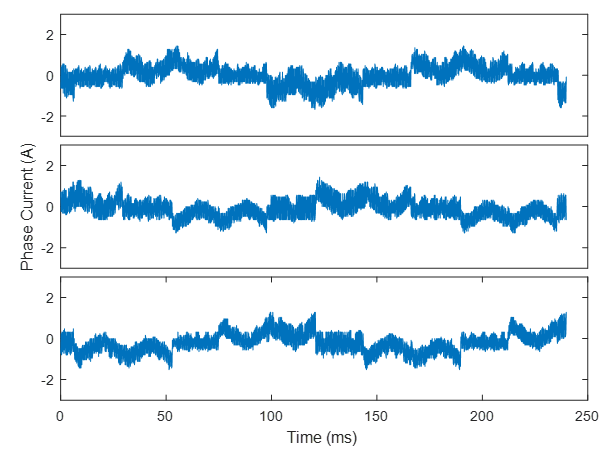
\includegraphics[clip,width=8cm]{Images/waveforms/trap_curr_1.png}%
	}

	\subfloat[Duty Cycle = 50\%\label{subfig-2:trap2c}]{%
  		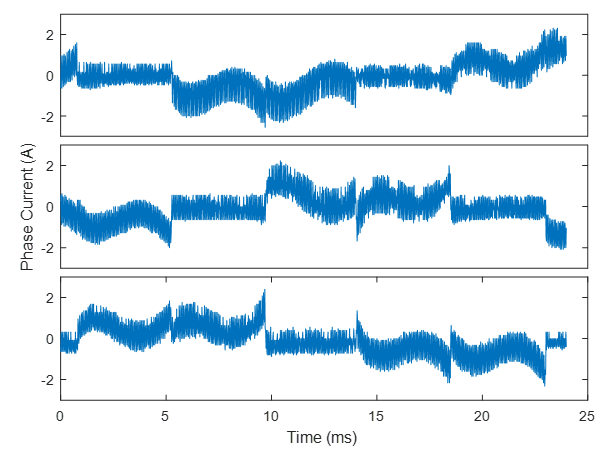
\includegraphics[clip,width=8cm]{Images/waveforms/trap_curr_2.png}%
	}

	\subfloat[Duty Cycle = 100\%\label{subfig-3:trap3c}]{%
  		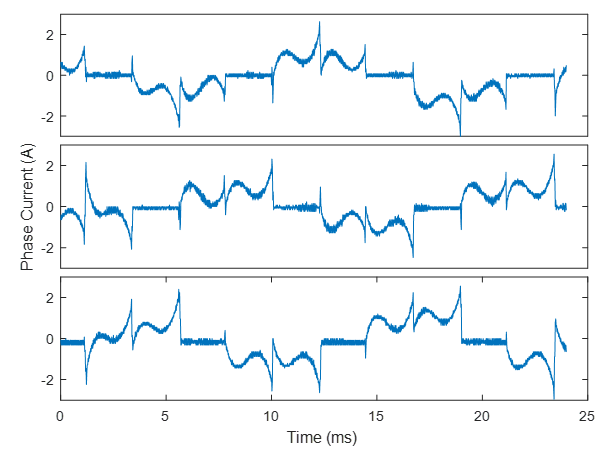
\includegraphics[clip,width=8cm]{Images/waveforms/trap_curr_3.png}%
	}
\caption{Trapezoidal drive current waveforms without load applied}
\label{fig:trap_c1}
\end{figure}

\begin{figure}[h!p]
\centering
	\subfloat[Duty Cycle = 10\%\label{subfig-1:trap4c}]{%
  		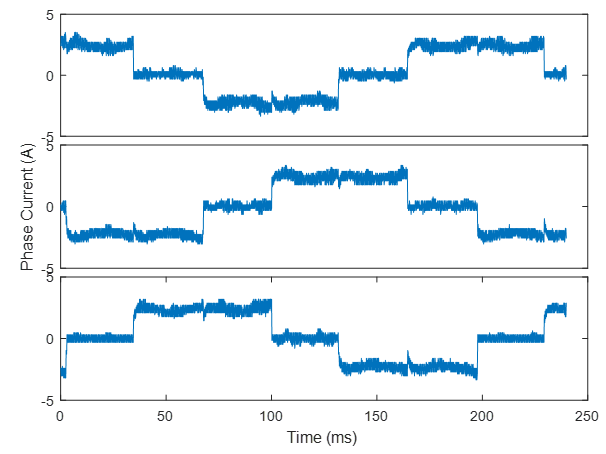
\includegraphics[clip,width=8cm]{Images/waveforms/trap_curr_4.png}%
	}

	\subfloat[Duty Cycle = 50\%\label{subfig-2:trap5c}]{%
  		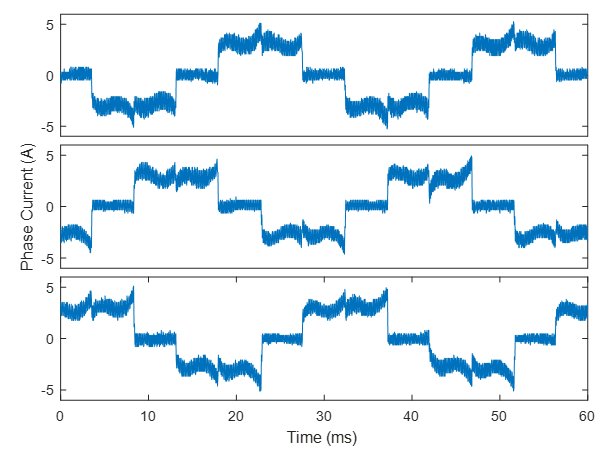
\includegraphics[clip,width=8cm]{Images/waveforms/trap_curr_5.png}%
	}

	\subfloat[Duty Cycle = 100\%\label{subfig-3:trap6c}]{%
  		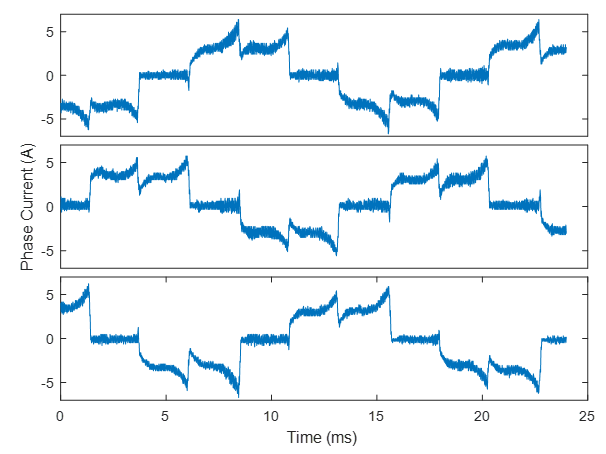
\includegraphics[clip,width=8cm]{Images/waveforms/trap_curr_6.png}%
	}
\caption{Trapezoidal drive current waveforms with load = 1 Nm}
\label{fig:trap_c2}
\end{figure}

\begin{figure}[h!p]
\centering
	\subfloat[Duty Cycle = 50\%\label{subfig-1:trap7c}]{%
  		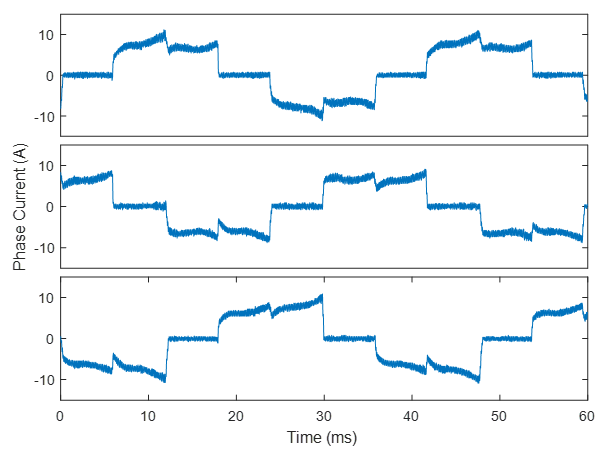
\includegraphics[clip,width=8cm]{Images/waveforms/trap_curr_7.png}%
	}

	\subfloat[Duty Cycle = 100\%\label{subfig-2:trap8c}]{%
  		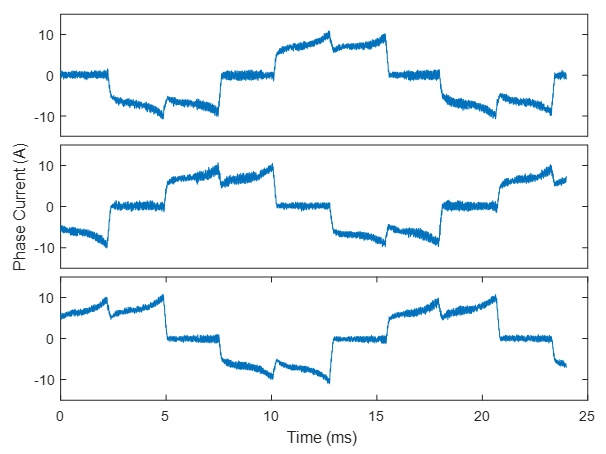
\includegraphics[clip,width=8cm]{Images/waveforms/trap_curr_8.png}%
	}
\caption{Trapezoidal drive current waveforms with load = 3 Nm}
\label{fig:trap_c3}
\end{figure}

\begin{figure}[h!p]
\centering
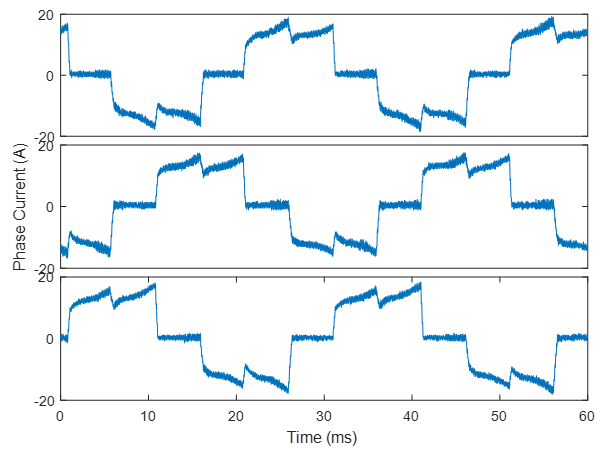
\includegraphics[width=8cm]{Images/waveforms/trap_curr_9.png} 
\caption[trapc9]{Trapezoidal drive current waveform with duty cycle = 70\% and load = 6 Nm}
\label{fig:trap_c4}
\end{figure}

\clearpage
\section{Speed Control with Trapezoidal Drive}

To see the behaviour of the speed control, different step signals were applied with different loads and different controller parameters. 

The torque loads were setup first at a steady speed to know the correct excitation voltage of the field, then the motor was stopped and step signal was applied.

Figures \ref{fig:plot2}, \ref{fig:plot3} and \ref{fig:plot4} show the different step responses between the same step signal applied and the same load but with different control parameters $K_{p}$ and $K_{i}$. It can be identified that, by changing the value of $K_{i}$ we obtain different damping behaviours on the motor.

In Figure \ref{fig:plot5} we compare two signals with different $K_{i}$ values, but in this case, in the test to obtain the signal with $K_{i} = 0.03$ the current was limited by the power supply. This shows that, even if $K_{i}$ is larger, the slew rate of the speed depends on the current limit of the power supply.

It is possible to see also the speed behaviour of the system compared with the duty cycle applied by the control algorithm on Figures \ref{fig:plot6} and \ref{fig:plot7}.

\begin{figure}[h!p]
\centering
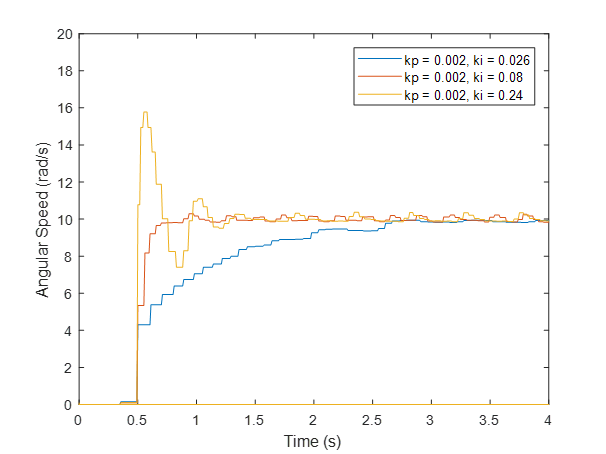
\includegraphics[width=10cm]{Images/plots/plot_2.png} 
\caption[Step response to a 10 rad/s signal without load applied]{Step response to a 10 rad/s signal without load applied}
\label{fig:plot2}
\end{figure}

\begin{figure}[h!p]
\centering
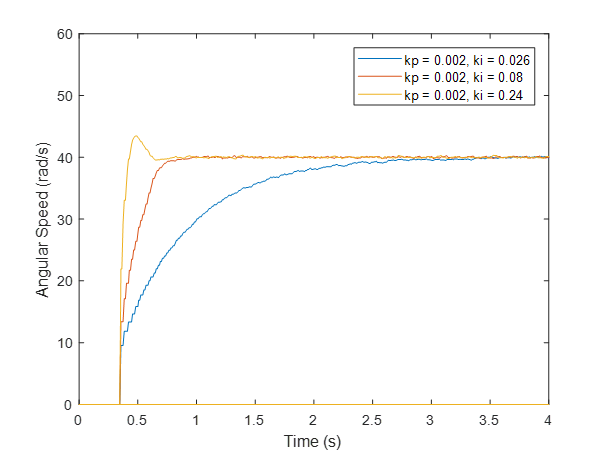
\includegraphics[width=10cm]{Images/plots/plot_3.png} 
\caption[Step response to a 40 rad/s signal without load applied]{Step response to a 40 rad/s signal without load applied}
\label{fig:plot3}
\end{figure}

\begin{figure}[h!p]
\centering
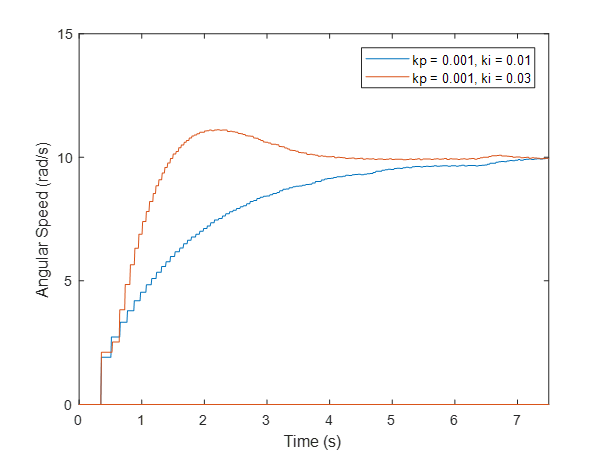
\includegraphics[width=10cm]{Images/plots/plot_4.png} 
\caption[Step response to a 10 rad/s signal with a 3 Nm load]{Step response to a 10 rad/s signal with a 3 Nm load}
\label{fig:plot4}
\end{figure}

\begin{figure}[h!p]
\centering
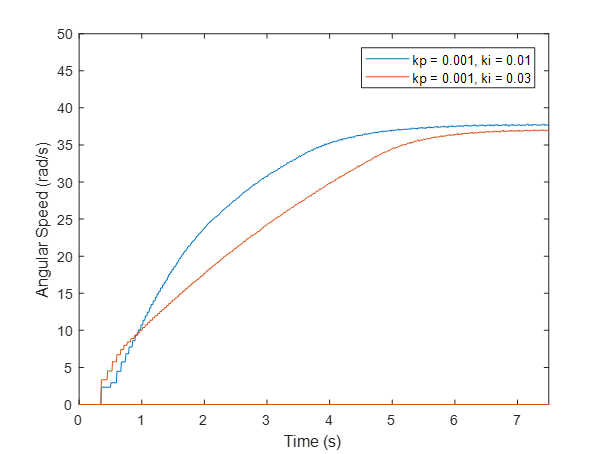
\includegraphics[width=10cm]{Images/plots/plot_5.png} 
\caption[Step response to a 40 rad/s signal with a 3 Nm load]{Step response to a 40 rad/s signal with a 3 Nm load}
\label{fig:plot5}
\end{figure}

\begin{figure}[h!p]
\centering
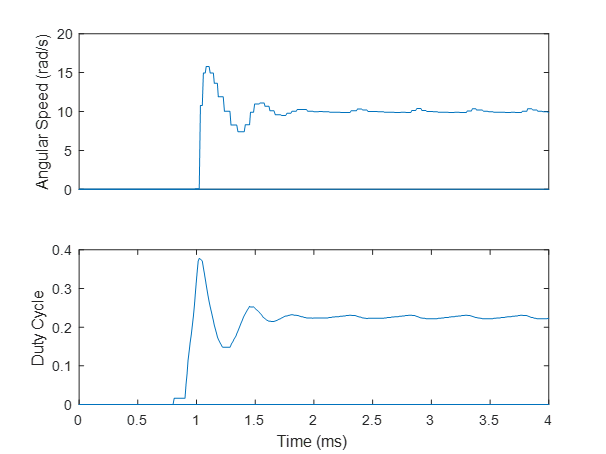
\includegraphics[width=10cm]{Images/plots/plot_6.png} 
\caption[Step response to a 10 rad/s signal without load, compared to its driving duty cycle signal]{Step response to a 10 rad/s signal without load, compared to its driving duty cycle signal}
\label{fig:plot6}
\end{figure}

\begin{figure}[h!p]
\centering
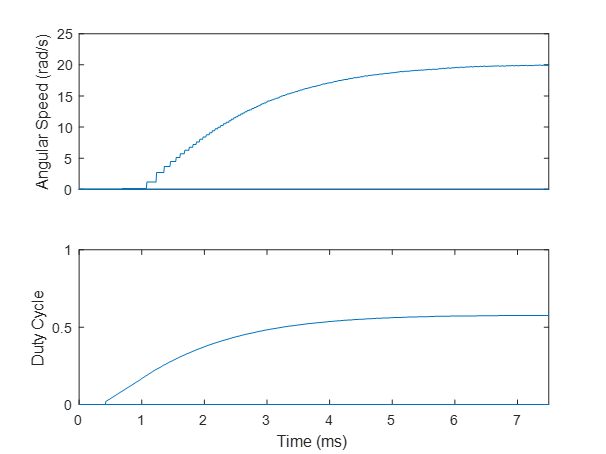
\includegraphics[width=10cm]{Images/plots/plot_7.png} 
\caption[Step response to a 20 rad/s signal with a 3 Nm load, compared to its driving duty cycle signal]{Step response to a 20 rad/s signal with a 3 Nm load, compared to its driving duty cycle signal}
\label{fig:plot7}
\end{figure}

\clearpage
\section{Sinusoidal Drive -- Open Loop}

This test was applied at the beginning of the development of the Field Oriented Control to test the generation of a sinusoidal waveform depending on the angular position of the rotor. The signals were generated by applying a constant amplitude value as a quadrature voltage without any load attached to the motor.

Figure \ref{fig:center_pwm} shows the center-aligned PWM signal generated by the inverter in the motor terminals. We can identify the ringing effect on the rising and falling edges but it has a small duration, therefore it can be neglected.

It can be appreciated in Figure \ref{subfig-3:sin3} that the current in the highest and lowest side of the signal are limited by the LEM current sensor of the measurement board at $20A$. While doing these tests, one wire of the measurement board started melting since it didn't have the required diameter for this amount of current. Also the LEM transducers became hot, since they were configured to measure signals of $\pm5A$ to provide a better resolution.

\begin{figure}[h!p]
\centering
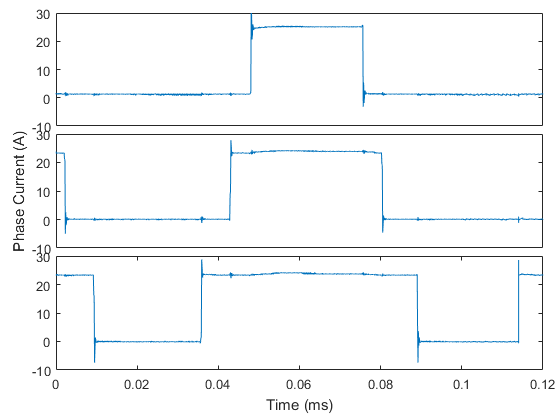
\includegraphics[width=10cm]{Images/waveforms/center_pwm.png} 
\caption[Center-aligned PWM voltage waveform]{Center-aligned PWM voltage waveform}
\label{fig:center_pwm}
\end{figure}

\begin{figure}[h!p]
\centering
	\subfloat[Quadrature voltage = 1V\label{subfig-1:sin1}]{%
  		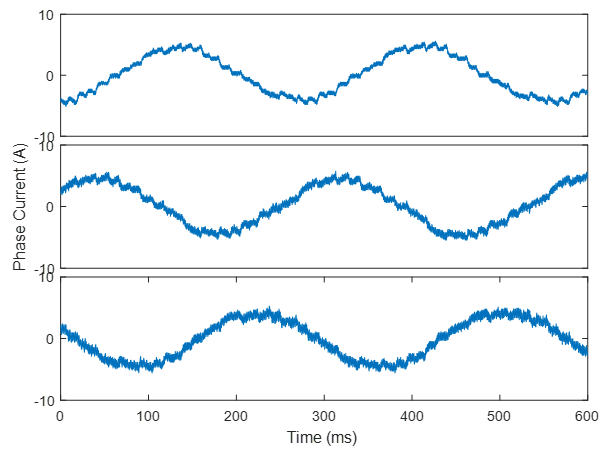
\includegraphics[clip,width=8cm]{Images/waveforms/sin1.png}%
	}

	\subfloat[Quadrature voltage = 2V\label{subfig-2:sin2}]{%
  		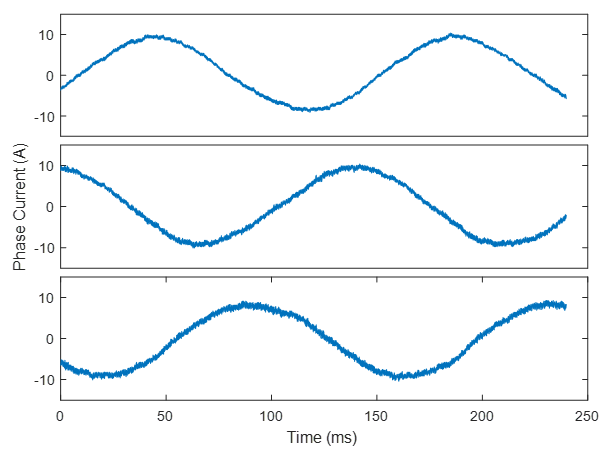
\includegraphics[clip,width=8cm]{Images/waveforms/sin2.png}%
	}

	\subfloat[Quadrature voltage = 5V\label{subfig-3:sin3}]{%
  		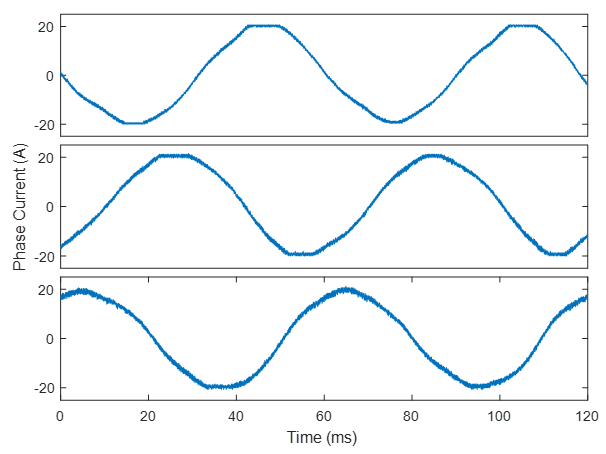
\includegraphics[clip,width=8cm]{Images/waveforms/sin3.png}%
	}
\caption{Sinusoidal drive current waveforms without load applied}
\end{figure}

\clearpage
\section{Field Oriented Control}

These tests were applied by exciting the field of the \ac{DC} generator to the maximum available ($30V$), so by setting up a reference quadrature current on the controller, the motor would reach a steady state speed when the torque applied by the load is equal to the torque applied by the motor.

The \ac{FOC} loop is executed at $10kHz$ due to the limitation imposed by the Orbis encoder.

From these tests we can compare the torque measured with the torque applied by multiplying the amplitude of the current waveform by the torque constant of the motor $K_{T}$ equal to $0.4506 Nm/A$. By doing this, we see that there is a loss of about 30\% of the torque on the tests with $1$ and $3 Nm$ loads, which can be due to mechanical losses and to measurement errors on the load torque. In the case when the load is $5 Nm$ the torque loss is around 50\%. We can identify that this current presents a distortion on its sinusoidal waveform and an offset of almost $1A$, which can be the reason of such power loss.

\begin{figure}[h!p]
\centering
	\subfloat[FOC signal with a 1 Nm load\label{subfig-1:sin4}]{%
  		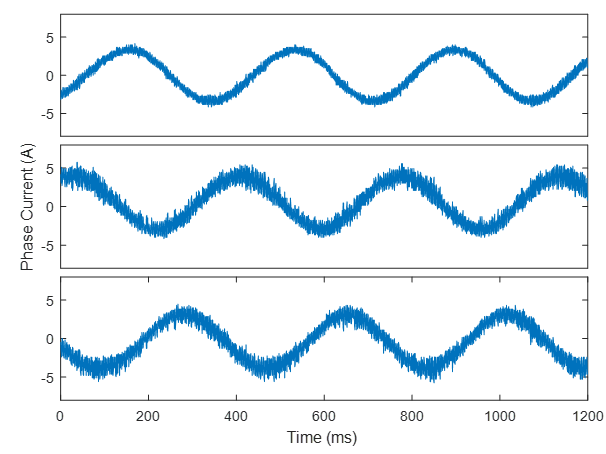
\includegraphics[width=5.5cm]{Images/waveforms/sin4.png}%
	}
\hfill
	\subfloat[FOC signal with a 3 Nm load\label{subfig-2:sin5}]{%
  		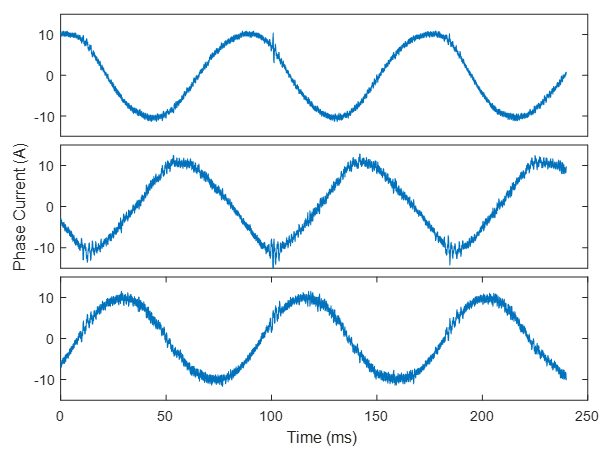
\includegraphics[width=5.5cm]{Images/waveforms/sin5.png}%
	}

	\subfloat[FOC signal with a 5 Nm load\label{subfig-3:sin6}]{%
  		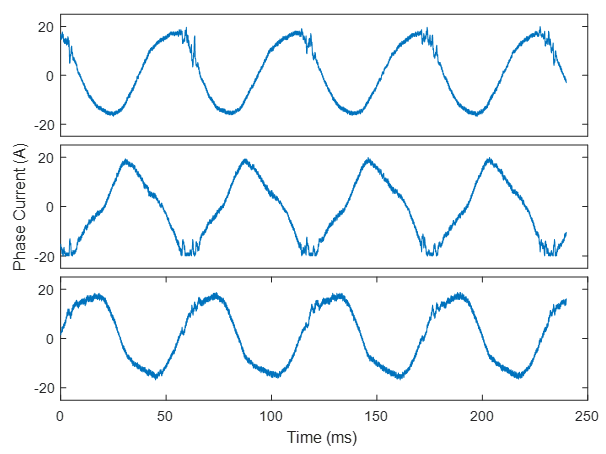
\includegraphics[width=10cm]{Images/waveforms/sin6.png}%
	}
\caption{FOC with different loads}
\end{figure}

\clearpage
\section{Speed Control with Field Oriented Control}

The behaviour of the driver with different reference speeds and load values can be appreciated from the remaining figures of this chapter.

By analysing the frequency of the waveform in Figure \ref{subfig-1:sin7} we can see the ability of the controller to move the motor at a low speed with a load applied.

It can be appreciated in Figures \ref{subfig-3:sin9}, \ref{subfig-3:sin12} and \ref{subfig-4:sin13} that the signal gets distorted when the speed reaches approximately $20rad/s$. This is due to the maximum frequency achievable by the Orbis encoder. Currently it represents a trade-off between the choosing the trapezoidal driven speed control, which works fine at high speeds since the angular position feedback is given by the hall effect sensors, and the \ac{FOC} driven speed control, which works fine at low speeds but at high speeds becomes unpredictable.

In order to have an idea of the linear speed achievable by the in-wheel motor, $20rad/s$ is equivalent to $9.1km/h$, which is approximately the human walking speed.

In Figure \ref{fig:plot8} we can see the comparison of the behaviour of the controller with the same step signal ($0$ to $10 rad/s$) but with different load. When the load is $3 Nm$, the slope of the signal becomes limited by the controller parameter \texttt{I\_MAX}, which defines the saturation of the integral part of the controller to avoid current peaks. This parameter can be modified accordingly to the capacities of the system, but caution must be taken since this can provoke malfunctioning of the circuit.

In figure \ref{fig:lastone} we can appreciate the three phase currents settling into steady state after a step signal is commanded to the controller.

\begin{figure}[h!p]
\centering
	\subfloat[5 rad/s\label{subfig-1:sin7}]{%
  		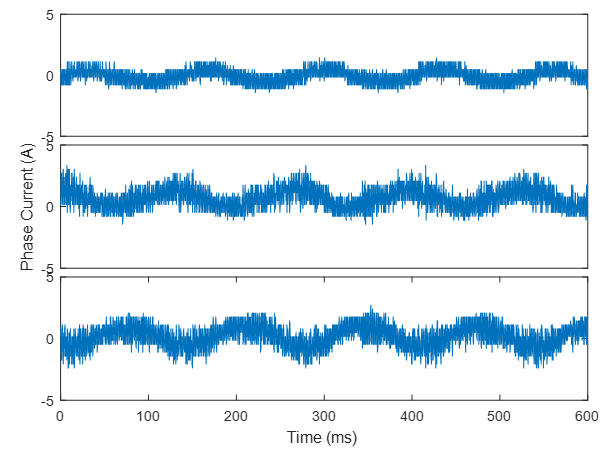
\includegraphics[clip,width=8cm]{Images/waveforms/sin7.png}%
	}

	\subfloat[20 rad/s\label{subfig-2:sin8}]{%
  		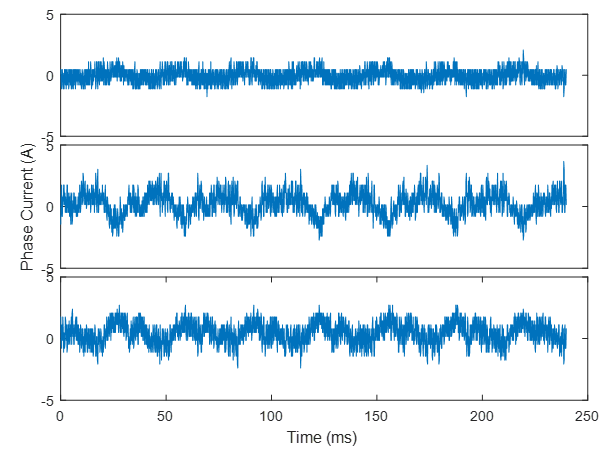
\includegraphics[clip,width=8cm]{Images/waveforms/sin8.png}%
	}

	\subfloat[40 rad/s\label{subfig-3:sin9}]{%
  		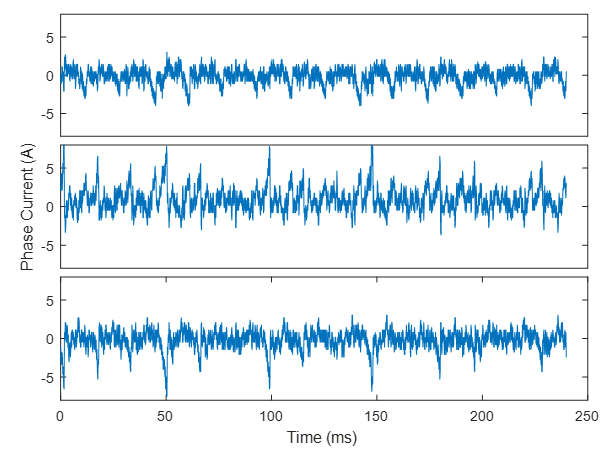
\includegraphics[clip,width=8cm]{Images/waveforms/sin9.png}%
	}
\caption{FOC speed control loop without load applied}
\end{figure}


\begin{figure}[h!p]
\centering
	\subfloat[1 rad/s\label{subfig-1:sin10}]{%
  		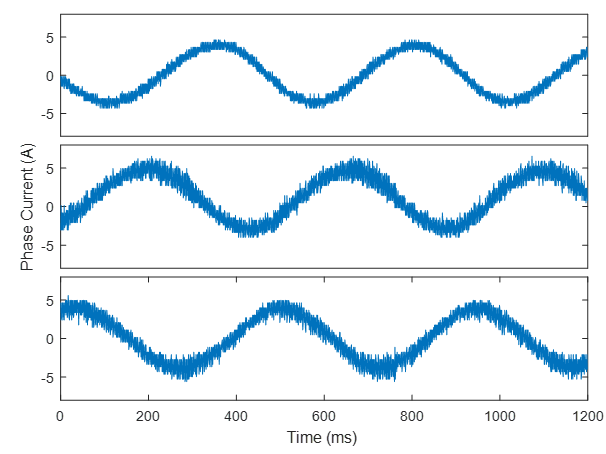
\includegraphics[width=5.5cm]{Images/waveforms/sin10.png}%
	}
	\hfill
	\subfloat[10 rad/s\label{subfig-2:sin11}]{%
  		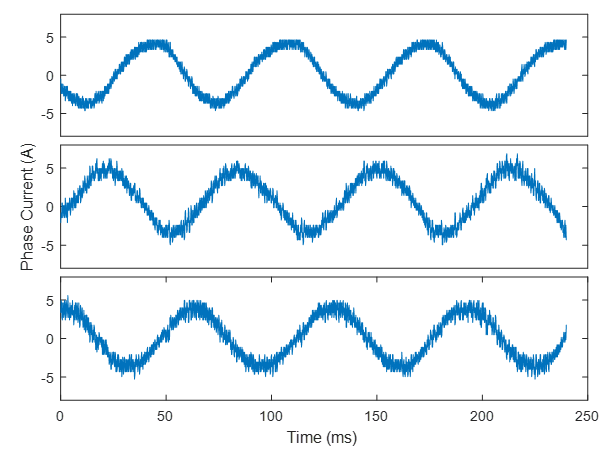
\includegraphics[width=5.5cm]{Images/waveforms/sin11.png}%
	}

	\subfloat[20 rad/s\label{subfig-3:sin12}]{%
  		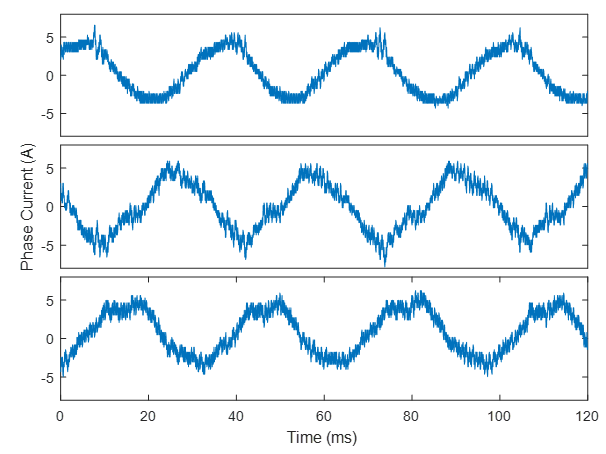
\includegraphics[width=5.5cm]{Images/waveforms/sin12.png}%
	}
	\hfill
	\subfloat[30 rad/s\label{subfig-4:sin13}]{%
  		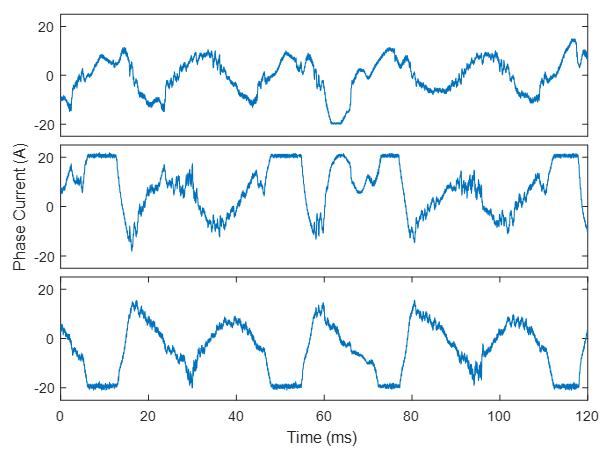
\includegraphics[width=5.5cm]{Images/waveforms/sin13.png}%
	}
\caption{FOC speed control loop with 1 Nm load}
\end{figure}

\begin{figure}[h!p]
\centering
	\subfloat[10 rad/s\label{subfig-1:sin14}]{%
  		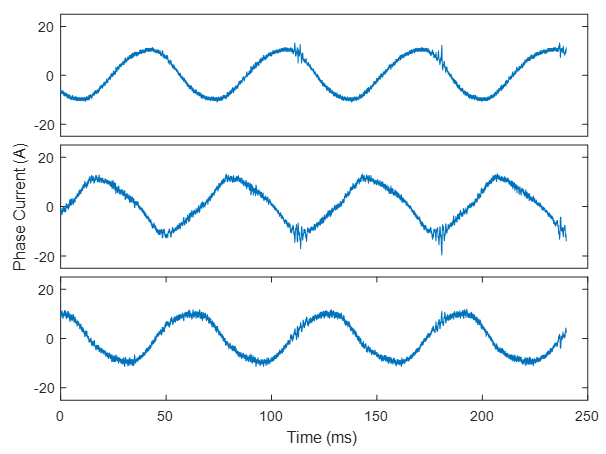
\includegraphics[clip,width=8cm]{Images/waveforms/sin14.png}%
	}

	\subfloat[20 rad/s\label{subfig-2:sin15}]{%
  		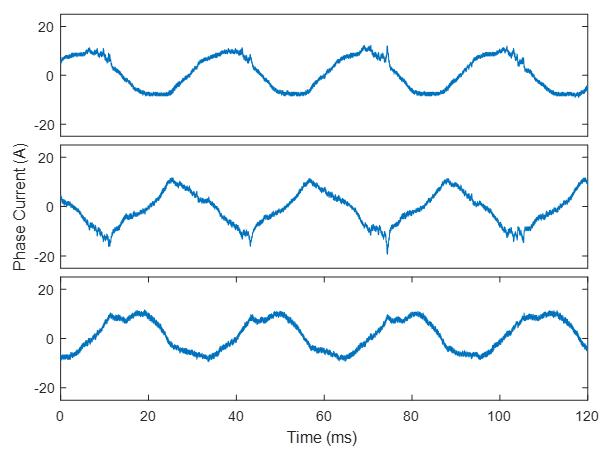
\includegraphics[clip,width=8cm]{Images/waveforms/sin15.png}%
	}
\caption{FOC speed control loop with 3 Nm load}
\end{figure}

\clearpage

\begin{figure}[h!p]
\centering
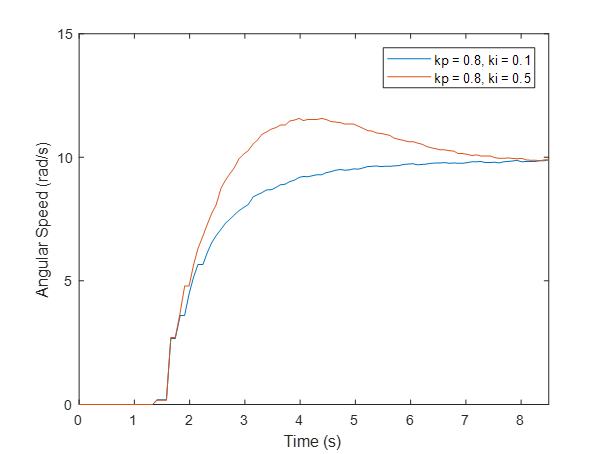
\includegraphics[width=10cm]{Images/plots/plot_8.png} 
\caption[plot8]{Step response to a 10 rad/s signal and a load of 1 Nm with different controller parameters}
\label{fig:plot8}
\end{figure}

\begin{figure}[h!p]
\centering
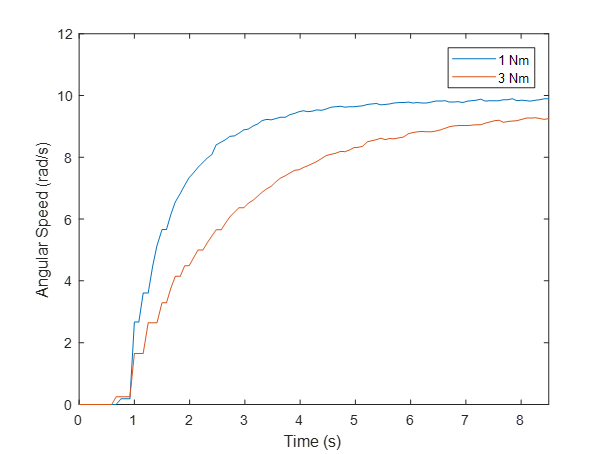
\includegraphics[width=10cm]{Images/plots/plot_9.png} 
\caption[plot9]{Step response to a 10 rad/s signal with different loads}
\label{fig:plot9}
\end{figure}

\clearpage

\begin{figure}[h!p]
\centering
	\subfloat[]{%
  		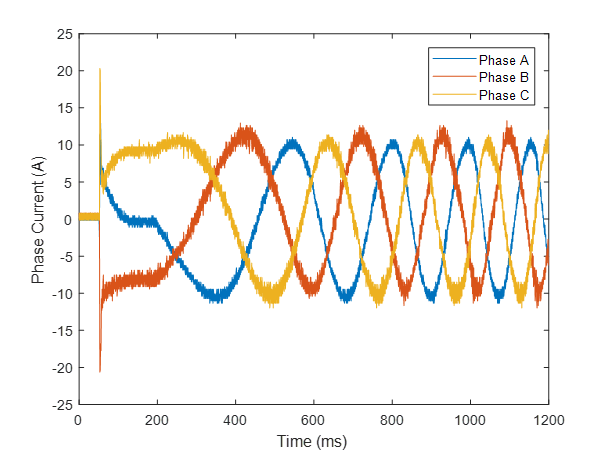
\includegraphics[clip,width=8.5cm]{Images/waveforms/sin20.png}%
	}

	\subfloat[]{%
  		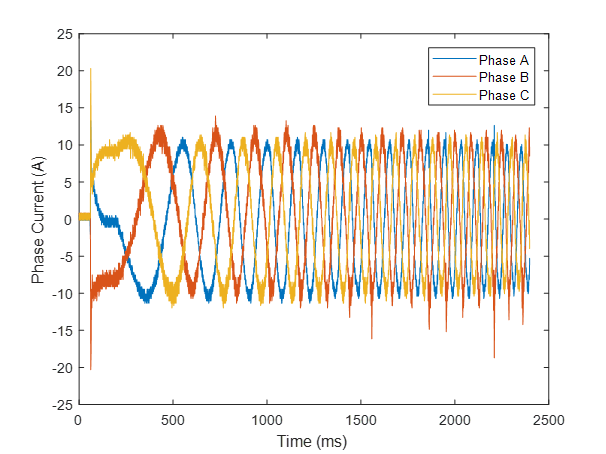
\includegraphics[clip,width=8.5cm]{Images/waveforms/sin19.png}%
	}

	\subfloat[]{%
  		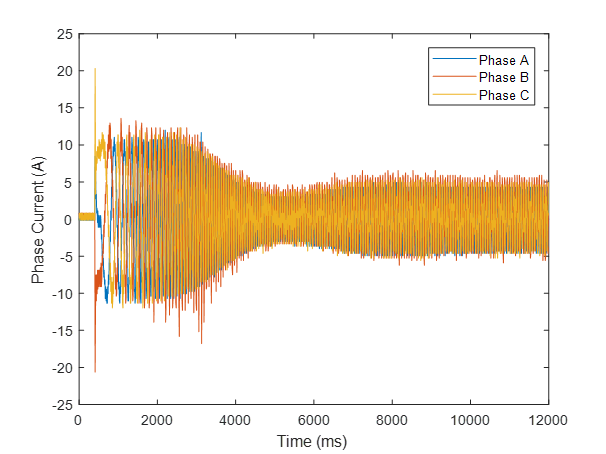
\includegraphics[clip,width=8.5cm]{Images/waveforms/sin18.png}%
	}
\caption{FOC three-phase current waveform in a step response to a 10 rad/s signal with a load of 1 Nm}
\label{fig:lastone}
\end{figure}